\documentclass[1p]{elsarticle_modified}
%\bibliographystyle{elsarticle-num}

%\usepackage[colorlinks]{hyperref}
%\usepackage{abbrmath_seonhwa} %\Abb, \Ascr, \Acal ,\Abf, \Afrak
\usepackage{amsfonts}
\usepackage{amssymb}
\usepackage{amsmath}
\usepackage{amsthm}
\usepackage{scalefnt}
\usepackage{amsbsy}
\usepackage{kotex}
\usepackage{caption}
\usepackage{subfig}
\usepackage{color}
\usepackage{graphicx}
\usepackage{xcolor} %% white, black, red, green, blue, cyan, magenta, yellow
\usepackage{float}
\usepackage{setspace}
\usepackage{hyperref}

\usepackage{tikz}
\usetikzlibrary{arrows}

\usepackage{multirow}
\usepackage{array} % fixed length table
\usepackage{hhline}

%%%%%%%%%%%%%%%%%%%%%
\makeatletter
\renewcommand*\env@matrix[1][\arraystretch]{%
	\edef\arraystretch{#1}%
	\hskip -\arraycolsep
	\let\@ifnextchar\new@ifnextchar
	\array{*\c@MaxMatrixCols c}}
\makeatother %https://tex.stackexchange.com/questions/14071/how-can-i-increase-the-line-spacing-in-a-matrix
%%%%%%%%%%%%%%%

\usepackage[normalem]{ulem}

\newcommand{\msout}[1]{\ifmmode\text{\sout{\ensuremath{#1}}}\else\sout{#1}\fi}
%SOURCE: \msout is \stkout macro in https://tex.stackexchange.com/questions/20609/strikeout-in-math-mode

\newcommand{\cancel}[1]{
	\ifmmode
	{\color{red}\msout{#1}}
	\else
	{\color{red}\sout{#1}}
	\fi
}

\newcommand{\add}[1]{
	{\color{blue}\uwave{#1}}
}

\newcommand{\replace}[2]{
	\ifmmode
	{\color{red}\msout{#1}}{\color{blue}\uwave{#2}}
	\else
	{\color{red}\sout{#1}}{\color{blue}\uwave{#2}}
	\fi
}

\newcommand{\Sol}{\mathcal{S}} %segment
\newcommand{\D}{D} %diagram
\newcommand{\A}{\mathcal{A}} %arc


%%%%%%%%%%%%%%%%%%%%%%%%%%%%%5 test

\def\sl{\operatorname{\textup{SL}}(2,\Cbb)}
\def\psl{\operatorname{\textup{PSL}}(2,\Cbb)}
\def\quan{\mkern 1mu \triangleright \mkern 1mu}

\theoremstyle{definition}
\newtheorem{thm}{Theorem}[section]
\newtheorem{prop}[thm]{Proposition}
\newtheorem{lem}[thm]{Lemma}
\newtheorem{ques}[thm]{Question}
\newtheorem{cor}[thm]{Corollary}
\newtheorem{defn}[thm]{Definition}
\newtheorem{exam}[thm]{Example}
\newtheorem{rmk}[thm]{Remark}
\newtheorem{alg}[thm]{Algorithm}

\newcommand{\I}{\sqrt{-1}}
\begin{document}

%\begin{frontmatter}
%
%\title{Boundary parabolic representations of knots up to 8 crossings}
%
%%% Group authors per affiliation:
%\author{Yunhi Cho} 
%\address{Department of Mathematics, University of Seoul, Seoul, Korea}
%\ead{yhcho@uos.ac.kr}
%
%
%\author{Seonhwa Kim} %\fnref{s_kim}}
%\address{Center for Geometry and Physics, Institute for Basic Science, Pohang, 37673, Korea}
%\ead{ryeona17@ibs.re.kr}
%
%\author{Hyuk Kim}
%\address{Department of Mathematical Sciences, Seoul National University, Seoul 08826, Korea}
%\ead{hyukkim@snu.ac.kr}
%
%\author{Seokbeom Yoon}
%\address{Department of Mathematical Sciences, Seoul National University, Seoul, 08826,  Korea}
%\ead{sbyoon15@snu.ac.kr}
%
%\begin{abstract}
%We find all boundary parabolic representation of knots up to 8 crossings.
%
%\end{abstract}
%\begin{keyword}
%    \MSC[2010] 57M25 
%\end{keyword}
%
%\end{frontmatter}

%\linenumbers
%\tableofcontents
%
\newcommand\colored[1]{\textcolor{white}{\rule[-0.35ex]{0.8em}{1.4ex}}\kern-0.8em\color{red} #1}%
%\newcommand\colored[1]{\textcolor{white}{ #1}\kern-2.17ex	\textcolor{white}{ #1}\kern-1.81ex	\textcolor{white}{ #1}\kern-2.15ex\color{red}#1	}

{\Large $\underline{12a_{0879}~(K12a_{0879})}$}

\setlength{\tabcolsep}{10pt}
\renewcommand{\arraystretch}{1.6}
\vspace{1cm}\begin{tabular}{m{100pt}>{\centering\arraybackslash}m{274pt}}
\multirow{5}{120pt}{
	\centering
	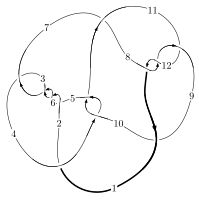
\includegraphics[width=112pt]{../../../GIT/diagram.site/Diagrams/png/1680_12a_0879.png}\\
\ \ \ A knot diagram\footnotemark}&
\allowdisplaybreaks
\textbf{Linearized knot diagam} \\
\cline{2-2}
 &
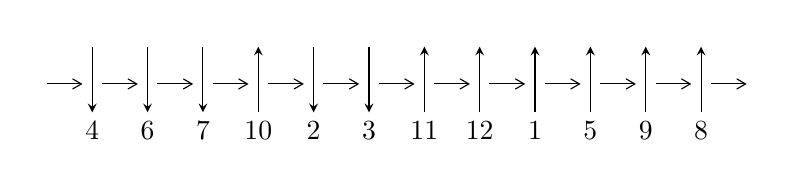
\begin{tikzpicture}[x=20pt, y=17pt]
	% nodes
	\node (C0) at (0, 0) {};
	\node (C1) at (1, 0) {};
	\node (C1U) at (1, +1) {};
	\node (C1D) at (1, -1) {4};

	\node (C2) at (2, 0) {};
	\node (C2U) at (2, +1) {};
	\node (C2D) at (2, -1) {6};

	\node (C3) at (3, 0) {};
	\node (C3U) at (3, +1) {};
	\node (C3D) at (3, -1) {7};

	\node (C4) at (4, 0) {};
	\node (C4U) at (4, +1) {};
	\node (C4D) at (4, -1) {10};

	\node (C5) at (5, 0) {};
	\node (C5U) at (5, +1) {};
	\node (C5D) at (5, -1) {2};

	\node (C6) at (6, 0) {};
	\node (C6U) at (6, +1) {};
	\node (C6D) at (6, -1) {3};

	\node (C7) at (7, 0) {};
	\node (C7U) at (7, +1) {};
	\node (C7D) at (7, -1) {11};

	\node (C8) at (8, 0) {};
	\node (C8U) at (8, +1) {};
	\node (C8D) at (8, -1) {12};

	\node (C9) at (9, 0) {};
	\node (C9U) at (9, +1) {};
	\node (C9D) at (9, -1) {1};

	\node (C10) at (10, 0) {};
	\node (C10U) at (10, +1) {};
	\node (C10D) at (10, -1) {5};

	\node (C11) at (11, 0) {};
	\node (C11U) at (11, +1) {};
	\node (C11D) at (11, -1) {9};

	\node (C12) at (12, 0) {};
	\node (C12U) at (12, +1) {};
	\node (C12D) at (12, -1) {8};
	\node (C13) at (13, 0) {};

	% arrows
	\draw[->,>={angle 60}]
	(C0) edge (C1) (C1) edge (C2) (C2) edge (C3) (C3) edge (C4) (C4) edge (C5) (C5) edge (C6) (C6) edge (C7) (C7) edge (C8) (C8) edge (C9) (C9) edge (C10) (C10) edge (C11) (C11) edge (C12) (C12) edge (C13) ;	\draw[->,>=stealth]
	(C1U) edge (C1D) (C2U) edge (C2D) (C3U) edge (C3D) (C4D) edge (C4U) (C5U) edge (C5D) (C6U) edge (C6D) (C7D) edge (C7U) (C8D) edge (C8U) (C9D) edge (C9U) (C10D) edge (C10U) (C11D) edge (C11U) (C12D) edge (C12U) ;
	\end{tikzpicture} \\
\hhline{~~} \\& 
\textbf{Solving Sequence} \\ \cline{2-2} 
 &
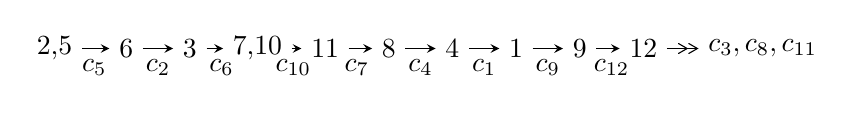
\begin{tikzpicture}[x=23pt, y=7pt]
	% node
	\node (A0) at (-1/8, 0) {2,5};
	\node (A1) at (1, 0) {6};
	\node (A2) at (2, 0) {3};
	\node (A3) at (49/16, 0) {7,10};
	\node (A4) at (33/8, 0) {11};
	\node (A5) at (41/8, 0) {8};
	\node (A6) at (49/8, 0) {4};
	\node (A7) at (57/8, 0) {1};
	\node (A8) at (65/8, 0) {9};
	\node (A9) at (73/8, 0) {12};
	\node (C1) at (1/2, -1) {$c_{5}$};
	\node (C2) at (3/2, -1) {$c_{2}$};
	\node (C3) at (5/2, -1) {$c_{6}$};
	\node (C4) at (29/8, -1) {$c_{10}$};
	\node (C5) at (37/8, -1) {$c_{7}$};
	\node (C6) at (45/8, -1) {$c_{4}$};
	\node (C7) at (53/8, -1) {$c_{1}$};
	\node (C8) at (61/8, -1) {$c_{9}$};
	\node (C9) at (69/8, -1) {$c_{12}$};
	\node (A10) at (11, 0) {$c_{3},c_{8},c_{11}$};

	% edge
	\draw[->,>=stealth]	
	(A0) edge (A1) (A1) edge (A2) (A2) edge (A3) (A3) edge (A4) (A4) edge (A5) (A5) edge (A6) (A6) edge (A7) (A7) edge (A8) (A8) edge (A9) ;
	\draw[->>,>={angle 60}]	
	(A9) edge (A10);
\end{tikzpicture} \\ 

\end{tabular} \\

\footnotetext{
The image of knot diagram is generated by the software ``\textbf{Draw programme}" developed by Andrew Bartholomew(\url{http://www.layer8.co.uk/maths/draw/index.htm\#Running-draw}), where we modified some parts for our purpose(\url{https://github.com/CATsTAILs/LinksPainter}).
}\phantom \\ \newline 
\centering \textbf{Ideals for irreducible components\footnotemark of $X_{\text{par}}$} 
 
\begin{align*}
I^u_{1}&=\langle 
-27 u^{65}-62 u^{64}+\cdots+2 b-19,\;65 u^{65}+146 u^{64}+\cdots+4 a+79,\;u^{66}+4 u^{65}+\cdots-7 u+1\rangle \\
I^u_{2}&=\langle 
b,\;a^3- a^2 u+a^2+2 u-3,\;u^2- u-1\rangle \\
\\
\end{align*}
\raggedright * 2 irreducible components of $\dim_{\mathbb{C}}=0$, with total 72 representations.\\
\footnotetext{All coefficients of polynomials are rational numbers. But the coefficients are sometimes approximated in decimal forms when there is not enough margin.}
\newpage
\renewcommand{\arraystretch}{1}
\centering \section*{I. $I^u_{1}= \langle -27 u^{65}-62 u^{64}+\cdots+2 b-19,\;65 u^{65}+146 u^{64}+\cdots+4 a+79,\;u^{66}+4 u^{65}+\cdots-7 u+1 \rangle$}
\flushleft \textbf{(i) Arc colorings}\\
\begin{tabular}{m{7pt} m{180pt} m{7pt} m{180pt} }
\flushright $a_{2}=$&$\begin{pmatrix}0\\u\end{pmatrix}$ \\
\flushright $a_{5}=$&$\begin{pmatrix}1\\0\end{pmatrix}$ \\
\flushright $a_{6}=$&$\begin{pmatrix}1\\u^2\end{pmatrix}$ \\
\flushright $a_{3}=$&$\begin{pmatrix}- u\\- u^3+u\end{pmatrix}$ \\
\flushright $a_{7}=$&$\begin{pmatrix}- u^2+1\\- u^4+2 u^2\end{pmatrix}$ \\
\flushright $a_{10}=$&$\begin{pmatrix}-16.2500 u^{65}-36.5000 u^{64}+\cdots+117.250 u-19.7500\\\frac{27}{2} u^{65}+31 u^{64}+\cdots-\frac{137}{2} u+\frac{19}{2}\end{pmatrix}$ \\
\flushright $a_{11}=$&$\begin{pmatrix}-2.75000 u^{65}-5.50000 u^{64}+\cdots+48.7500 u-10.2500\\\frac{27}{2} u^{65}+31 u^{64}+\cdots-\frac{137}{2} u+\frac{19}{2}\end{pmatrix}$ \\
\flushright $a_{8}=$&$\begin{pmatrix}-\frac{1}{4} u^{64}-\frac{3}{4} u^{63}+\cdots+\frac{3}{2} u+\frac{9}{4}\\- u^9+5 u^7-7 u^5+2 u^3- u\end{pmatrix}$ \\
\flushright $a_{4}=$&$\begin{pmatrix}u^3-2 u\\u^5-3 u^3+u\end{pmatrix}$ \\
\flushright $a_{1}=$&$\begin{pmatrix}u^7-4 u^5+4 u^3\\u^9-5 u^7+7 u^5-2 u^3+u\end{pmatrix}$ \\
\flushright $a_{9}=$&$\begin{pmatrix}-12.5000 u^{65}-27.2500 u^{64}+\cdots+97.5000 u-17.2500\\\frac{21}{4} u^{65}+\frac{49}{4} u^{64}+\cdots-\frac{113}{4} u+4\end{pmatrix}$ \\
\flushright $a_{12}=$&$\begin{pmatrix}-3 u^{65}-\frac{19}{4} u^{64}+\cdots+27 u-\frac{19}{4}\\\frac{1}{4} u^{65}+\frac{1}{2} u^{64}+\cdots-\frac{3}{4} u+\frac{1}{4}\end{pmatrix}$\\&\end{tabular}
\flushleft \textbf{(ii) Obstruction class $= -1$}\\~\\
\flushleft \textbf{(iii) Cusp Shapes $= -23 u^{65}-59 u^{64}+\cdots+\frac{175}{2} u+\frac{5}{2}$}\\~\\
\newpage\renewcommand{\arraystretch}{1}
\flushleft \textbf{(iv) u-Polynomials at the component}\newline \\
\begin{tabular}{m{50pt}|m{274pt}}
Crossings & \hspace{64pt}u-Polynomials at each crossing \\
\hline $$\begin{aligned}c_{1}\end{aligned}$$&$\begin{aligned}
&u^{66}-16 u^{65}+\cdots-7063 u-529
\end{aligned}$\\
\hline $$\begin{aligned}c_{2},c_{3},c_{5}\\c_{6}\end{aligned}$$&$\begin{aligned}
&u^{66}+4 u^{65}+\cdots-7 u+1
\end{aligned}$\\
\hline $$\begin{aligned}c_{4},c_{10}\end{aligned}$$&$\begin{aligned}
&u^{66}- u^{65}+\cdots-32 u-64
\end{aligned}$\\
\hline $$\begin{aligned}c_{7},c_{9}\end{aligned}$$&$\begin{aligned}
&u^{66}-3 u^{65}+\cdots+394 u-241
\end{aligned}$\\
\hline $$\begin{aligned}c_{8},c_{11},c_{12}\end{aligned}$$&$\begin{aligned}
&u^{66}+3 u^{65}+\cdots-2 u-1
\end{aligned}$\\
\hline
\end{tabular}\\~\\
\newpage\renewcommand{\arraystretch}{1}
\flushleft \textbf{(v) Riley Polynomials at the component}\newline \\
\begin{tabular}{m{50pt}|m{274pt}}
Crossings & \hspace{64pt}Riley Polynomials at each crossing \\
\hline $$\begin{aligned}c_{1}\end{aligned}$$&$\begin{aligned}
&y^{66}+8 y^{65}+\cdots-58875795 y+279841
\end{aligned}$\\
\hline $$\begin{aligned}c_{2},c_{3},c_{5}\\c_{6}\end{aligned}$$&$\begin{aligned}
&y^{66}-76 y^{65}+\cdots-39 y+1
\end{aligned}$\\
\hline $$\begin{aligned}c_{4},c_{10}\end{aligned}$$&$\begin{aligned}
&y^{66}-35 y^{65}+\cdots-87040 y+4096
\end{aligned}$\\
\hline $$\begin{aligned}c_{7},c_{9}\end{aligned}$$&$\begin{aligned}
&y^{66}-45 y^{65}+\cdots+1824338 y+58081
\end{aligned}$\\
\hline $$\begin{aligned}c_{8},c_{11},c_{12}\end{aligned}$$&$\begin{aligned}
&y^{66}+55 y^{65}+\cdots+26 y+1
\end{aligned}$\\
\hline
\end{tabular}\\~\\
\newpage\flushleft \textbf{(vi) Complex Volumes and Cusp Shapes}
$$\begin{array}{c|c|c}  
\text{Solutions to }I^u_{1}& \I (\text{vol} + \sqrt{-1}CS) & \text{Cusp shape}\\
 \hline 
\begin{aligned}
u &= -1.072920 + 0.173234 I \\
a &= \phantom{-}0.033699 - 0.206753 I \\
b &= -1.156190 + 0.223934 I\end{aligned}
 & -1.68039 - 4.13387 I & \phantom{-0.000000 } 0 \\ \hline\begin{aligned}
u &= -1.072920 - 0.173234 I \\
a &= \phantom{-}0.033699 + 0.206753 I \\
b &= -1.156190 - 0.223934 I\end{aligned}
 & -1.68039 + 4.13387 I & \phantom{-0.000000 } 0 \\ \hline\begin{aligned}
u &= \phantom{-}0.690848 + 0.580355 I \\
a &= \phantom{-}1.60685 + 1.18393 I \\
b &= -1.265350 + 0.605450 I\end{aligned}
 & \phantom{-}1.32088 - 11.43940 I & \phantom{-0.000000 } 0 \\ \hline\begin{aligned}
u &= \phantom{-}0.690848 - 0.580355 I \\
a &= \phantom{-}1.60685 - 1.18393 I \\
b &= -1.265350 - 0.605450 I\end{aligned}
 & \phantom{-}1.32088 + 11.43940 I & \phantom{-0.000000 } 0 \\ \hline\begin{aligned}
u &= \phantom{-}0.664269 + 0.585797 I \\
a &= -1.63457 - 1.15491 I \\
b &= \phantom{-}1.281820 - 0.540344 I\end{aligned}
 & \phantom{-}5.90981 - 7.14877 I & \phantom{-0.000000 } 0 \\ \hline\begin{aligned}
u &= \phantom{-}0.664269 - 0.585797 I \\
a &= -1.63457 + 1.15491 I \\
b &= \phantom{-}1.281820 + 0.540344 I\end{aligned}
 & \phantom{-}5.90981 + 7.14877 I & \phantom{-0.000000 } 0 \\ \hline\begin{aligned}
u &= \phantom{-}0.625394 + 0.587261 I \\
a &= \phantom{-}1.67658 + 1.11501 I \\
b &= -1.286450 + 0.445199 I\end{aligned}
 & \phantom{-}2.78876 - 2.77757 I & \phantom{-0.000000 } 0 \\ \hline\begin{aligned}
u &= \phantom{-}0.625394 - 0.587261 I \\
a &= \phantom{-}1.67658 - 1.11501 I \\
b &= -1.286450 - 0.445199 I\end{aligned}
 & \phantom{-}2.78876 + 2.77757 I & \phantom{-0.000000 } 0 \\ \hline\begin{aligned}
u &= -0.749842 + 0.310450 I \\
a &= \phantom{-}0.324495 + 0.129177 I \\
b &= \phantom{-}0.649778 - 0.650531 I\end{aligned}
 & -5.73446 + 0.49899 I & -5.69937 - 1.38908 I \\ \hline\begin{aligned}
u &= -0.749842 - 0.310450 I \\
a &= \phantom{-}0.324495 - 0.129177 I \\
b &= \phantom{-}0.649778 + 0.650531 I\end{aligned}
 & -5.73446 - 0.49899 I & -5.69937 + 1.38908 I\\
 \hline 
 \end{array}$$\newpage$$\begin{array}{c|c|c}  
\text{Solutions to }I^u_{1}& \I (\text{vol} + \sqrt{-1}CS) & \text{Cusp shape}\\
 \hline 
\begin{aligned}
u &= -1.189200 + 0.068111 I \\
a &= -0.238134 + 0.114543 I \\
b &= \phantom{-}1.228180 - 0.049346 I\end{aligned}
 & \phantom{-}2.35220 - 0.00558 I & \phantom{-0.000000 } 0 \\ \hline\begin{aligned}
u &= -1.189200 - 0.068111 I \\
a &= -0.238134 - 0.114543 I \\
b &= \phantom{-}1.228180 + 0.049346 I\end{aligned}
 & \phantom{-}2.35220 + 0.00558 I & \phantom{-0.000000 } 0 \\ \hline\begin{aligned}
u &= \phantom{-}0.646920 + 0.426476 I \\
a &= -1.85311 - 1.39072 I \\
b &= \phantom{-}0.922593 - 0.479193 I\end{aligned}
 & -4.87688 - 4.92488 I & -2.91516 + 7.92049 I \\ \hline\begin{aligned}
u &= \phantom{-}0.646920 - 0.426476 I \\
a &= -1.85311 + 1.39072 I \\
b &= \phantom{-}0.922593 + 0.479193 I\end{aligned}
 & -4.87688 + 4.92488 I & -2.91516 - 7.92049 I \\ \hline\begin{aligned}
u &= \phantom{-}0.325420 + 0.652249 I \\
a &= -1.70719 - 0.69127 I \\
b &= \phantom{-}1.302590 + 0.277842 I\end{aligned}
 & \phantom{-}3.67408 - 1.40819 I & \phantom{-}4.92934 + 2.83994 I \\ \hline\begin{aligned}
u &= \phantom{-}0.325420 - 0.652249 I \\
a &= -1.70719 + 0.69127 I \\
b &= \phantom{-}1.302590 - 0.277842 I\end{aligned}
 & \phantom{-}3.67408 + 1.40819 I & \phantom{-}4.92934 - 2.83994 I \\ \hline\begin{aligned}
u &= \phantom{-}0.547891 + 0.477188 I \\
a &= \phantom{-}1.92682 + 1.12711 I \\
b &= -1.034770 + 0.276618 I\end{aligned}
 & \phantom{-}1.07485 - 3.31172 I & \phantom{-}3.02602 + 8.16126 I \\ \hline\begin{aligned}
u &= \phantom{-}0.547891 - 0.477188 I \\
a &= \phantom{-}1.92682 - 1.12711 I \\
b &= -1.034770 - 0.276618 I\end{aligned}
 & \phantom{-}1.07485 + 3.31172 I & \phantom{-}3.02602 - 8.16126 I \\ \hline\begin{aligned}
u &= -0.550846 + 0.473180 I \\
a &= -0.638662 - 0.120591 I \\
b &= -0.283002 + 1.026680 I\end{aligned}
 & -1.79557 + 5.51844 I & -0.23058 - 6.89017 I \\ \hline\begin{aligned}
u &= -0.550846 - 0.473180 I \\
a &= -0.638662 + 0.120591 I \\
b &= -0.283002 - 1.026680 I\end{aligned}
 & -1.79557 - 5.51844 I & -0.23058 + 6.89017 I\\
 \hline 
 \end{array}$$\newpage$$\begin{array}{c|c|c}  
\text{Solutions to }I^u_{1}& \I (\text{vol} + \sqrt{-1}CS) & \text{Cusp shape}\\
 \hline 
\begin{aligned}
u &= \phantom{-}0.281335 + 0.666408 I \\
a &= \phantom{-}1.67352 + 0.63814 I \\
b &= -1.291680 - 0.386170 I\end{aligned}
 & \phantom{-}7.04097 + 2.92886 I & \phantom{-}8.20980 - 1.22760 I \\ \hline\begin{aligned}
u &= \phantom{-}0.281335 - 0.666408 I \\
a &= \phantom{-}1.67352 - 0.63814 I \\
b &= -1.291680 + 0.386170 I\end{aligned}
 & \phantom{-}7.04097 - 2.92886 I & \phantom{-}8.20980 + 1.22760 I \\ \hline\begin{aligned}
u &= \phantom{-}0.246514 + 0.675439 I \\
a &= -1.64567 - 0.59911 I \\
b &= \phantom{-}1.274070 + 0.469465 I\end{aligned}
 & \phantom{-}2.63500 + 7.21380 I & \phantom{-}3.80665 - 3.88169 I \\ \hline\begin{aligned}
u &= \phantom{-}0.246514 - 0.675439 I \\
a &= -1.64567 + 0.59911 I \\
b &= \phantom{-}1.274070 - 0.469465 I\end{aligned}
 & \phantom{-}2.63500 - 7.21380 I & \phantom{-}3.80665 + 3.88169 I \\ \hline\begin{aligned}
u &= -1.318540 + 0.118766 I \\
a &= \phantom{-}0.453383 - 0.293355 I \\
b &= -1.314510 - 0.011883 I\end{aligned}
 & -1.46349 + 4.26617 I & \phantom{-0.000000 } 0 \\ \hline\begin{aligned}
u &= -1.318540 - 0.118766 I \\
a &= \phantom{-}0.453383 + 0.293355 I \\
b &= -1.314510 + 0.011883 I\end{aligned}
 & -1.46349 - 4.26617 I & \phantom{-0.000000 } 0 \\ \hline\begin{aligned}
u &= -0.488537 + 0.457113 I \\
a &= \phantom{-}0.700481 + 0.055283 I \\
b &= \phantom{-}0.160120 - 0.986891 I\end{aligned}
 & \phantom{-}2.36817 + 1.61935 I & \phantom{-}5.06499 - 4.29154 I \\ \hline\begin{aligned}
u &= -0.488537 - 0.457113 I \\
a &= \phantom{-}0.700481 - 0.055283 I \\
b &= \phantom{-}0.160120 + 0.986891 I\end{aligned}
 & \phantom{-}2.36817 - 1.61935 I & \phantom{-}5.06499 + 4.29154 I \\ \hline\begin{aligned}
u &= -0.604078 + 0.148414 I \\
a &= -0.253436 + 0.106782 I \\
b &= -0.286923 + 0.422139 I\end{aligned}
 & -1.106760 + 0.360302 I & -7.12806 - 1.59413 I \\ \hline\begin{aligned}
u &= -0.604078 - 0.148414 I \\
a &= -0.253436 - 0.106782 I \\
b &= -0.286923 - 0.422139 I\end{aligned}
 & -1.106760 - 0.360302 I & -7.12806 + 1.59413 I\\
 \hline 
 \end{array}$$\newpage$$\begin{array}{c|c|c}  
\text{Solutions to }I^u_{1}& \I (\text{vol} + \sqrt{-1}CS) & \text{Cusp shape}\\
 \hline 
\begin{aligned}
u &= -0.403566 + 0.462584 I \\
a &= -0.820575 - 0.001706 I \\
b &= \phantom{-}0.001443 + 0.972652 I\end{aligned}
 & -1.36002 - 2.20380 I & \phantom{-}1.274205 - 0.508380 I \\ \hline\begin{aligned}
u &= -0.403566 - 0.462584 I \\
a &= -0.820575 + 0.001706 I \\
b &= \phantom{-}0.001443 - 0.972652 I\end{aligned}
 & -1.36002 + 2.20380 I & \phantom{-}1.274205 + 0.508380 I \\ \hline\begin{aligned}
u &= \phantom{-}0.407492 + 0.444561 I \\
a &= -2.10136 - 0.83022 I \\
b &= \phantom{-}0.941571 - 0.012463 I\end{aligned}
 & \phantom{-}1.50011 + 0.02255 I & \phantom{-}5.79860 + 0.11054 I \\ \hline\begin{aligned}
u &= \phantom{-}0.407492 - 0.444561 I \\
a &= -2.10136 + 0.83022 I \\
b &= \phantom{-}0.941571 + 0.012463 I\end{aligned}
 & \phantom{-}1.50011 - 0.02255 I & \phantom{-}5.79860 - 0.11054 I \\ \hline\begin{aligned}
u &= \phantom{-}0.446019 + 0.205803 I \\
a &= \phantom{-}3.01031 + 1.00239 I \\
b &= -0.585824 + 0.096244 I\end{aligned}
 & -3.60533 + 2.43505 I & \phantom{-}4.47869 + 3.50639 I \\ \hline\begin{aligned}
u &= \phantom{-}0.446019 - 0.205803 I \\
a &= \phantom{-}3.01031 - 1.00239 I \\
b &= -0.585824 - 0.096244 I\end{aligned}
 & -3.60533 - 2.43505 I & \phantom{-}4.47869 - 3.50639 I \\ \hline\begin{aligned}
u &= \phantom{-}1.51687 + 0.09420 I \\
a &= \phantom{-}0.265118 + 0.603915 I \\
b &= \phantom{-}0.284104 + 1.091710 I\end{aligned}
 & -7.76260 + 0.42615 I & \phantom{-0.000000 } 0 \\ \hline\begin{aligned}
u &= \phantom{-}1.51687 - 0.09420 I \\
a &= \phantom{-}0.265118 - 0.603915 I \\
b &= \phantom{-}0.284104 - 1.091710 I\end{aligned}
 & -7.76260 - 0.42615 I & \phantom{-0.000000 } 0 \\ \hline\begin{aligned}
u &= -1.52878 + 0.09849 I \\
a &= \phantom{-}1.127160 - 0.797641 I \\
b &= -1.075640 - 0.324127 I\end{aligned}
 & -5.04567 + 1.71176 I & \phantom{-0.000000 } 0 \\ \hline\begin{aligned}
u &= -1.52878 - 0.09849 I \\
a &= \phantom{-}1.127160 + 0.797641 I \\
b &= -1.075640 + 0.324127 I\end{aligned}
 & -5.04567 - 1.71176 I & \phantom{-0.000000 } 0\\
 \hline 
 \end{array}$$\newpage$$\begin{array}{c|c|c}  
\text{Solutions to }I^u_{1}& \I (\text{vol} + \sqrt{-1}CS) & \text{Cusp shape}\\
 \hline 
\begin{aligned}
u &= \phantom{-}1.53900 + 0.11695 I \\
a &= -0.336179 - 0.567584 I \\
b &= -0.393546 - 1.106990 I\end{aligned}
 & -4.45170 - 3.60064 I & \phantom{-0.000000 } 0 \\ \hline\begin{aligned}
u &= \phantom{-}1.53900 - 0.11695 I \\
a &= -0.336179 + 0.567584 I \\
b &= -0.393546 + 1.106990 I\end{aligned}
 & -4.45170 + 3.60064 I & \phantom{-0.000000 } 0 \\ \hline\begin{aligned}
u &= -1.54855 + 0.07058 I \\
a &= -1.41831 + 0.83959 I \\
b &= \phantom{-}0.944998 + 0.301189 I\end{aligned}
 & -10.50730 - 1.36159 I & \phantom{-0.000000 } 0 \\ \hline\begin{aligned}
u &= -1.54855 - 0.07058 I \\
a &= -1.41831 - 0.83959 I \\
b &= \phantom{-}0.944998 - 0.301189 I\end{aligned}
 & -10.50730 + 1.36159 I & \phantom{-0.000000 } 0 \\ \hline\begin{aligned}
u &= -1.55067 + 0.13221 I \\
a &= -0.959087 + 0.994864 I \\
b &= \phantom{-}1.134420 + 0.460428 I\end{aligned}
 & -5.97241 + 5.48876 I & \phantom{-0.000000 } 0 \\ \hline\begin{aligned}
u &= -1.55067 - 0.13221 I \\
a &= -0.959087 - 0.994864 I \\
b &= \phantom{-}1.134420 - 0.460428 I\end{aligned}
 & -5.97241 - 5.48876 I & \phantom{-0.000000 } 0 \\ \hline\begin{aligned}
u &= \phantom{-}1.55509 + 0.13012 I \\
a &= \phantom{-}0.379992 + 0.543053 I \\
b &= \phantom{-}0.471872 + 1.119230 I\end{aligned}
 & -8.88354 - 7.66796 I & \phantom{-0.000000 } 0 \\ \hline\begin{aligned}
u &= \phantom{-}1.55509 - 0.13012 I \\
a &= \phantom{-}0.379992 - 0.543053 I \\
b &= \phantom{-}0.471872 - 1.119230 I\end{aligned}
 & -8.88354 + 7.66796 I & \phantom{-0.000000 } 0 \\ \hline\begin{aligned}
u &= \phantom{-}0.061635 + 0.421413 I \\
a &= \phantom{-}1.80766 + 0.02094 I \\
b &= -0.645194 - 0.497522 I\end{aligned}
 & -3.43044 + 2.02248 I & \phantom{-}1.43635 - 3.15758 I \\ \hline\begin{aligned}
u &= \phantom{-}0.061635 - 0.421413 I \\
a &= \phantom{-}1.80766 - 0.02094 I \\
b &= -0.645194 + 0.497522 I\end{aligned}
 & -3.43044 - 2.02248 I & \phantom{-}1.43635 + 3.15758 I\\
 \hline 
 \end{array}$$\newpage$$\begin{array}{c|c|c}  
\text{Solutions to }I^u_{1}& \I (\text{vol} + \sqrt{-1}CS) & \text{Cusp shape}\\
 \hline 
\begin{aligned}
u &= -1.57094 + 0.17640 I \\
a &= -0.738128 + 1.094960 I \\
b &= \phantom{-}1.267420 + 0.596203 I\end{aligned}
 & -4.54503 + 5.58353 I & \phantom{-0.000000 } 0 \\ \hline\begin{aligned}
u &= -1.57094 - 0.17640 I \\
a &= -0.738128 - 1.094960 I \\
b &= \phantom{-}1.267420 - 0.596203 I\end{aligned}
 & -4.54503 - 5.58353 I & \phantom{-0.000000 } 0 \\ \hline\begin{aligned}
u &= \phantom{-}1.58225 + 0.03832 I \\
a &= \phantom{-}0.163322 + 0.361601 I \\
b &= \phantom{-}0.266777 + 0.702013 I\end{aligned}
 & -8.64237 - 1.04768 I & \phantom{-0.000000 } 0 \\ \hline\begin{aligned}
u &= \phantom{-}1.58225 - 0.03832 I \\
a &= \phantom{-}0.163322 - 0.361601 I \\
b &= \phantom{-}0.266777 - 0.702013 I\end{aligned}
 & -8.64237 + 1.04768 I & \phantom{-0.000000 } 0 \\ \hline\begin{aligned}
u &= -1.58571 + 0.12589 I \\
a &= \phantom{-}0.99022 - 1.21656 I \\
b &= -1.044450 - 0.580460 I\end{aligned}
 & -12.4486 + 6.9737 I & \phantom{-0.000000 } 0 \\ \hline\begin{aligned}
u &= -1.58571 - 0.12589 I \\
a &= \phantom{-}0.99022 + 1.21656 I \\
b &= -1.044450 + 0.580460 I\end{aligned}
 & -12.4486 - 6.9737 I & \phantom{-0.000000 } 0 \\ \hline\begin{aligned}
u &= -1.58854 + 0.17927 I \\
a &= \phantom{-}0.712511 - 1.165440 I \\
b &= -1.26100 - 0.66919 I\end{aligned}
 & -1.64539 + 9.99256 I & \phantom{-0.000000 } 0 \\ \hline\begin{aligned}
u &= -1.58854 - 0.17927 I \\
a &= \phantom{-}0.712511 + 1.165440 I \\
b &= -1.26100 + 0.66919 I\end{aligned}
 & -1.64539 - 9.99256 I & \phantom{-0.000000 } 0 \\ \hline\begin{aligned}
u &= -1.59986 + 0.17767 I \\
a &= -0.704976 + 1.212660 I \\
b &= \phantom{-}1.24315 + 0.71519 I\end{aligned}
 & -6.3848 + 14.2753 I & \phantom{-0.000000 } 0 \\ \hline\begin{aligned}
u &= -1.59986 - 0.17767 I \\
a &= -0.704976 - 1.212660 I \\
b &= \phantom{-}1.24315 - 0.71519 I\end{aligned}
 & -6.3848 - 14.2753 I & \phantom{-0.000000 } 0\\
 \hline 
 \end{array}$$\newpage$$\begin{array}{c|c|c}  
\text{Solutions to }I^u_{1}& \I (\text{vol} + \sqrt{-1}CS) & \text{Cusp shape}\\
 \hline 
\begin{aligned}
u &= \phantom{-}1.61738 + 0.07768 I \\
a &= -0.344588 - 0.328731 I \\
b &= -0.607410 - 0.737385 I\end{aligned}
 & -13.86580 - 1.91791 I & \phantom{-0.000000 } 0 \\ \hline\begin{aligned}
u &= \phantom{-}1.61738 - 0.07768 I \\
a &= -0.344588 + 0.328731 I \\
b &= -0.607410 + 0.737385 I\end{aligned}
 & -13.86580 + 1.91791 I & \phantom{-0.000000 } 0 \\ \hline\begin{aligned}
u &= \phantom{-}1.66435\phantom{ +0.000000I} \\
a &= -0.362345\phantom{ +0.000000I} \\
b &= -0.777375\phantom{ +0.000000I}\end{aligned}
 & -7.02502\phantom{ +0.000000I} & \phantom{-0.000000 } 0 \\ \hline\begin{aligned}
u &= \phantom{-}1.66975 + 0.02246 I \\
a &= \phantom{-}0.391254 + 0.078239 I \\
b &= \phantom{-}0.840309 + 0.197273 I\end{aligned}
 & -11.05450 + 3.59857 I & \phantom{-0.000000 } 0 \\ \hline\begin{aligned}
u &= \phantom{-}1.66975 - 0.02246 I \\
a &= \phantom{-}0.391254 - 0.078239 I \\
b &= \phantom{-}0.840309 - 0.197273 I\end{aligned}
 & -11.05450 - 3.59857 I & \phantom{-0.000000 } 0 \\ \hline\begin{aligned}
u &= \phantom{-}0.188647\phantom{ +0.000000I} \\
a &= -3.33648\phantom{ +0.000000I} \\
b &= \phantom{-}0.410787\phantom{ +0.000000I}\end{aligned}
 & \phantom{-}0.829449\phantom{ +0.000000I} & \phantom{-}12.8870\phantom{ +0.000000I}\\
 \hline 
 \end{array}$$\newpage\newpage\renewcommand{\arraystretch}{1}
\centering \section*{II. $I^u_{2}= \langle b,\;a^3- a^2 u+a^2+2 u-3,\;u^2- u-1 \rangle$}
\flushleft \textbf{(i) Arc colorings}\\
\begin{tabular}{m{7pt} m{180pt} m{7pt} m{180pt} }
\flushright $a_{2}=$&$\begin{pmatrix}0\\u\end{pmatrix}$ \\
\flushright $a_{5}=$&$\begin{pmatrix}1\\0\end{pmatrix}$ \\
\flushright $a_{6}=$&$\begin{pmatrix}1\\u+1\end{pmatrix}$ \\
\flushright $a_{3}=$&$\begin{pmatrix}- u\\- u-1\end{pmatrix}$ \\
\flushright $a_{7}=$&$\begin{pmatrix}- u\\- u\end{pmatrix}$ \\
\flushright $a_{10}=$&$\begin{pmatrix}a\\0\end{pmatrix}$ \\
\flushright $a_{11}=$&$\begin{pmatrix}a\\0\end{pmatrix}$ \\
\flushright $a_{8}=$&$\begin{pmatrix}- a^2 u- u\\- u\end{pmatrix}$ \\
\flushright $a_{4}=$&$\begin{pmatrix}1\\0\end{pmatrix}$ \\
\flushright $a_{1}=$&$\begin{pmatrix}u\\u\end{pmatrix}$ \\
\flushright $a_{9}=$&$\begin{pmatrix}a u+2 a\\a u+a\end{pmatrix}$ \\
\flushright $a_{12}=$&$\begin{pmatrix}-3 a^2 u- a^2+a+2 u-1\\-2 a^2 u- a^2+u\end{pmatrix}$\\&\end{tabular}
\flushleft \textbf{(ii) Obstruction class $= 1$}\\~\\
\flushleft \textbf{(iii) Cusp Shapes $= - a^2-2 a u+a- u-3$}\\~\\
\newpage\renewcommand{\arraystretch}{1}
\flushleft \textbf{(iv) u-Polynomials at the component}\newline \\
\begin{tabular}{m{50pt}|m{274pt}}
Crossings & \hspace{64pt}u-Polynomials at each crossing \\
\hline $$\begin{aligned}c_{1},c_{2},c_{3}\end{aligned}$$&$\begin{aligned}
&(u^2+u-1)^3
\end{aligned}$\\
\hline $$\begin{aligned}c_{4},c_{10}\end{aligned}$$&$\begin{aligned}
&u^6
\end{aligned}$\\
\hline $$\begin{aligned}c_{5},c_{6}\end{aligned}$$&$\begin{aligned}
&(u^2- u-1)^3
\end{aligned}$\\
\hline $$\begin{aligned}c_{7},c_{9}\end{aligned}$$&$\begin{aligned}
&(u^3- u^2+1)^2
\end{aligned}$\\
\hline $$\begin{aligned}c_{8}\end{aligned}$$&$\begin{aligned}
&(u^3+u^2+2 u+1)^2
\end{aligned}$\\
\hline $$\begin{aligned}c_{11},c_{12}\end{aligned}$$&$\begin{aligned}
&(u^3- u^2+2 u-1)^2
\end{aligned}$\\
\hline
\end{tabular}\\~\\
\newpage\renewcommand{\arraystretch}{1}
\flushleft \textbf{(v) Riley Polynomials at the component}\newline \\
\begin{tabular}{m{50pt}|m{274pt}}
Crossings & \hspace{64pt}Riley Polynomials at each crossing \\
\hline $$\begin{aligned}c_{1},c_{2},c_{3}\\c_{5},c_{6}\end{aligned}$$&$\begin{aligned}
&(y^2-3 y+1)^3
\end{aligned}$\\
\hline $$\begin{aligned}c_{4},c_{10}\end{aligned}$$&$\begin{aligned}
&y^6
\end{aligned}$\\
\hline $$\begin{aligned}c_{7},c_{9}\end{aligned}$$&$\begin{aligned}
&(y^3- y^2+2 y-1)^2
\end{aligned}$\\
\hline $$\begin{aligned}c_{8},c_{11},c_{12}\end{aligned}$$&$\begin{aligned}
&(y^3+3 y^2+2 y-1)^2
\end{aligned}$\\
\hline
\end{tabular}\\~\\
\newpage\flushleft \textbf{(vi) Complex Volumes and Cusp Shapes}
$$\begin{array}{c|c|c}  
\text{Solutions to }I^u_{2}& \I (\text{vol} + \sqrt{-1}CS) & \text{Cusp shape}\\
 \hline 
\begin{aligned}
u &= -0.618034\phantom{ +0.000000I} \\
a &= \phantom{-}1.22142\phantom{ +0.000000I} \\
b &= \phantom{-0.000000 } 0\end{aligned}
 & \phantom{-}0.126494\phantom{ +0.000000I} & -1.14270\phantom{ +0.000000I} \\ \hline\begin{aligned}
u &= -0.618034\phantom{ +0.000000I} \\
a &= -1.41973 + 1.20521 I \\
b &= \phantom{-0.000000 } 0\end{aligned}
 & -4.01109 - 2.82812 I & -6.11966 + 6.11708 I \\ \hline\begin{aligned}
u &= -0.618034\phantom{ +0.000000I} \\
a &= -1.41973 - 1.20521 I \\
b &= \phantom{-0.000000 } 0\end{aligned}
 & -4.01109 + 2.82812 I & -6.11966 - 6.11708 I \\ \hline\begin{aligned}
u &= \phantom{-}1.61803\phantom{ +0.000000I} \\
a &= \phantom{-}0.542287 + 0.460350 I \\
b &= \phantom{-0.000000 } 0\end{aligned}
 & -11.90680 + 2.82812 I & -5.91278 - 1.52866 I \\ \hline\begin{aligned}
u &= \phantom{-}1.61803\phantom{ +0.000000I} \\
a &= \phantom{-}0.542287 - 0.460350 I \\
b &= \phantom{-0.000000 } 0\end{aligned}
 & -11.90680 - 2.82812 I & -5.91278 + 1.52866 I \\ \hline\begin{aligned}
u &= \phantom{-}1.61803\phantom{ +0.000000I} \\
a &= -0.466540\phantom{ +0.000000I} \\
b &= \phantom{-0.000000 } 0\end{aligned}
 & -7.76919\phantom{ +0.000000I} & -3.79250\phantom{ +0.000000I}\\
 \hline 
 \end{array}$$\newpage
\newpage\renewcommand{\arraystretch}{1}
\centering \section*{ III. u-Polynomials}
\begin{tabular}{m{50pt}|m{274pt}}
Crossings & \hspace{64pt}u-Polynomials at each crossing \\
\hline $$\begin{aligned}c_{1}\end{aligned}$$&$\begin{aligned}
&((u^2+u-1)^3)(u^{66}-16 u^{65}+\cdots-7063 u-529)
\end{aligned}$\\
\hline $$\begin{aligned}c_{2},c_{3}\end{aligned}$$&$\begin{aligned}
&((u^2+u-1)^3)(u^{66}+4 u^{65}+\cdots-7 u+1)
\end{aligned}$\\
\hline $$\begin{aligned}c_{4},c_{10}\end{aligned}$$&$\begin{aligned}
&u^6(u^{66}- u^{65}+\cdots-32 u-64)
\end{aligned}$\\
\hline $$\begin{aligned}c_{5},c_{6}\end{aligned}$$&$\begin{aligned}
&((u^2- u-1)^3)(u^{66}+4 u^{65}+\cdots-7 u+1)
\end{aligned}$\\
\hline $$\begin{aligned}c_{7},c_{9}\end{aligned}$$&$\begin{aligned}
&((u^3- u^2+1)^2)(u^{66}-3 u^{65}+\cdots+394 u-241)
\end{aligned}$\\
\hline $$\begin{aligned}c_{8}\end{aligned}$$&$\begin{aligned}
&((u^3+u^2+2 u+1)^2)(u^{66}+3 u^{65}+\cdots-2 u-1)
\end{aligned}$\\
\hline $$\begin{aligned}c_{11},c_{12}\end{aligned}$$&$\begin{aligned}
&((u^3- u^2+2 u-1)^2)(u^{66}+3 u^{65}+\cdots-2 u-1)
\end{aligned}$\\
\hline
\end{tabular}\newpage\renewcommand{\arraystretch}{1}
\centering \section*{ IV. Riley Polynomials}
\begin{tabular}{m{50pt}|m{274pt}}
Crossings & \hspace{64pt}Riley Polynomials at each crossing \\
\hline $$\begin{aligned}c_{1}\end{aligned}$$&$\begin{aligned}
&((y^2-3 y+1)^3)(y^{66}+8 y^{65}+\cdots-5.88758\times10^{7} y+279841)
\end{aligned}$\\
\hline $$\begin{aligned}c_{2},c_{3},c_{5}\\c_{6}\end{aligned}$$&$\begin{aligned}
&((y^2-3 y+1)^3)(y^{66}-76 y^{65}+\cdots-39 y+1)
\end{aligned}$\\
\hline $$\begin{aligned}c_{4},c_{10}\end{aligned}$$&$\begin{aligned}
&y^6(y^{66}-35 y^{65}+\cdots-87040 y+4096)
\end{aligned}$\\
\hline $$\begin{aligned}c_{7},c_{9}\end{aligned}$$&$\begin{aligned}
&((y^3- y^2+2 y-1)^2)(y^{66}-45 y^{65}+\cdots+1824338 y+58081)
\end{aligned}$\\
\hline $$\begin{aligned}c_{8},c_{11},c_{12}\end{aligned}$$&$\begin{aligned}
&((y^3+3 y^2+2 y-1)^2)(y^{66}+55 y^{65}+\cdots+26 y+1)
\end{aligned}$\\
\hline
\end{tabular}
\vskip 2pc
\end{document}